\documentclass{article}
\usepackage[utf8]{inputenc}
\usepackage[brazilian]{babel}
\usepackage{url}
\usepackage{graphicx}
\usepackage{geometry}
\usepackage{enumitem}
\usepackage{float}
\usepackage{amsmath}
\usepackage[table,xcdraw]{xcolor}

\geometry{a4paper, left=20mm, right=20mm, top=20mm, bottom=20mm}
 

\begin{document}

\begin{frame}{}
    \hspace*{-0.5cm}
    $\vcenter{\hbox{
\includegraphics[width=1cm]{mackenzie-logo.png}}}$
    $\vcenter{\resizebox{0.95\textwidth}{!}{
        \begin{tabular}{c}
          Leandro N. de Castro \& Daniel Ferrari  \\
          Introdução à Mineração de Dados: Conceitos Básicos, Algoritmos e Aplicações \\
             \hline 
             Marcos Cordeiro de Brito Jr
        \end{tabular}
    }}$
\end{frame}

\begin{center}
  \huge \textbf{CADERNO DE EXERCÍCIOS – PARTE 02} \\ 
\end{center}

\setcounter{section}{4}
\section{CAPÍTULO 05: CLASSIFICAÇÃO DE DADOS}
\subsection{EXERCÍCIOS CONCEITUAIS}
\subsubsection{Durante o desenvolvimento de um modelo de classificação a base de dados é dividida em dois conjuntos. Quais são estes conjuntos e qual é o propósito desta separação}
\textit{Resposta:} 

\subsubsection{Discuta por quê para bases de dados reais na maioria das vezes treinar um sistema preditivo até que o erro para os dados de treinamento seja zero não é aconselhável.}
\textit{Resposta:}

\subsubsection{O que é a validação cruzada em k-pastas? Qual é a sua finalidade?}
\textit{Resposta:} 

\subsubsection{O que é a matriz de confusão de um problema de classificação binária? Explique os quatro valores apresentados pela matriz.}
\textit{Resposta:} 

\subsection{EXERCÍCIOS NUMÉRICOS}

\subsubsection{Utilizando a árvore de decisão para o conjunto de treinamento da base de dados Cogumelos, apresentada na Figura 5.19, extraia todas as regras de classificação para cogumelos venenosos.}
\textit{Resposta:} 

\subsubsection{Considere o seguinte problema: Um determinado algoritmo é responsável por indicar se um paciente está doente ou não. Após a realização de um experimento com 150 pacientes, onde 30 estavam doentes, o algoritmo informou a existência de 28 doentes sendo que 8 destes estavam saudáveis. Calcule a taxa de verdadeiro positivo \textit{(TPR)}, a taxa de falso positivo \textit{(FPR)}, a acurácia  \textit{(ACC)}, e a precisão \textit{(Pr)}.}
\textit{Resposta:} 

\subsubsection{Construa uma árvore de decisão para a base de dados abaixo.}
\begin{figure}[H]
    \centering 
    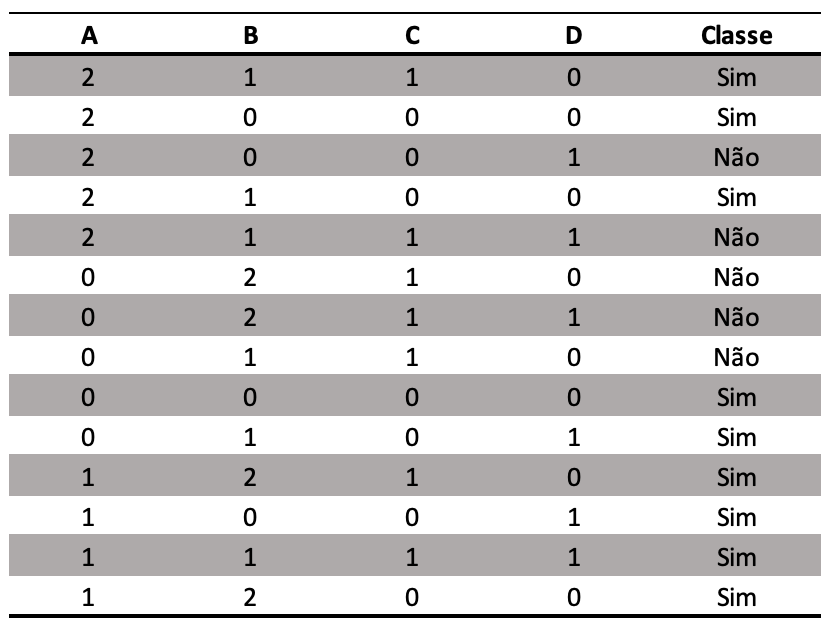
\includegraphics[width=8cm]{tab-5-2-3.png} 
  \end{figure}

\textit{Resposta:} 

\subsubsection{Aplique o classificador \textit{Naïve Bayes} na base de dados abaixo e determine o valor para classe \textbf{Jogar} dos seguintes objetos:}
\begin{enumerate}[label=\alph*]
    \item X = (Ensolarado, Branda, Alta, Não)
    \item Y = (Chuvoso, Fria, Alta, Sim)
    \item Z = (Ensolarado, Branda, Normal, Não)
    \item W = (Fechado , Fria, Normal, Sim)
\end{enumerate}

\begin{figure}[H]
    \centering 
    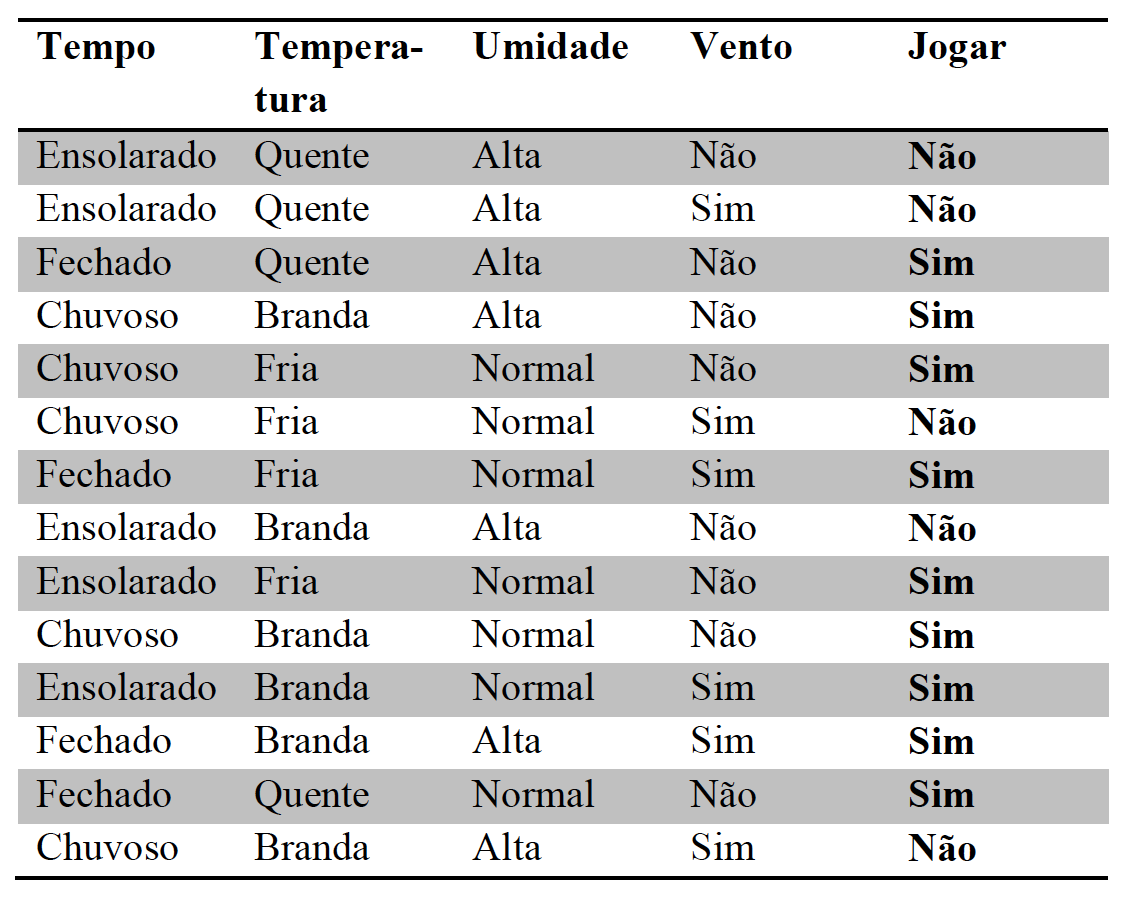
\includegraphics[width=8cm]{tab-5-2-4.png} 
  \end{figure}

\textit{Resposta:} 

\end{document}